\chapter{Resultados}
\label{cap:results}

\section{RQ1. Com que frequência \textit{breaking changes} impactam nos pacotes clientes?}

Nesta Seção, encontram-se os resultados da análise manual voltados para responder a primeira questão de pesquisa. Nessa Seção estão os dados relacionados à quantificação das \textit{breaking changes}.

\subsubsection{\textbf{10.4\% dos clientes e 8.4\% das \textit{releases} sofreram \textit{breaking changes}}}

De todos os 384 clientes que tiveram seus testes executados, 40 (10.4\%) apresentaram algum caso de \textit{breaking changes}. Entretanto, os clientes podem ser impactados por mais de um tipo de erro, por exemplo, uma \textit{release} pode ser impactada por uma \textit{breaking change} e outra, por um erro interno. Assim, o mesmo cliente pode ser classificado em dois, ou mais, tipos de erros. Por isso, os resultados são melhores apresentados em função das \textit{releases}, uma vez que uma \textit{release} só pode ser impactada por apenas um tipo de erro. Desta maneira, analisando as \textit{releases}, de todas as \textit{2300} que tiveram seus testes executados, 902 (39.5\%) sofreram algum tipo de erro, que foram:

\begin{itemize}
    \item 433 (18.7\%) das \textit{releases} foram impactadas por erros internos;
    \item os casos particulares de \textit{breaking changes} impactaram 213 (9.2\%) das \textit{releases};
    \item as \textit{breaking changes} impactaram 193 (8.4\%) \textit{releases}; e
    \item 73 (3.2\%) das \textit{releases} foram impactadas por algum erro que não foi descoberto.
\end{itemize}{}

A Figura \ref{fig:pre_res_rq1} contém os resultados em função das \textit{releases}.

\begin{figure}
    \centering
    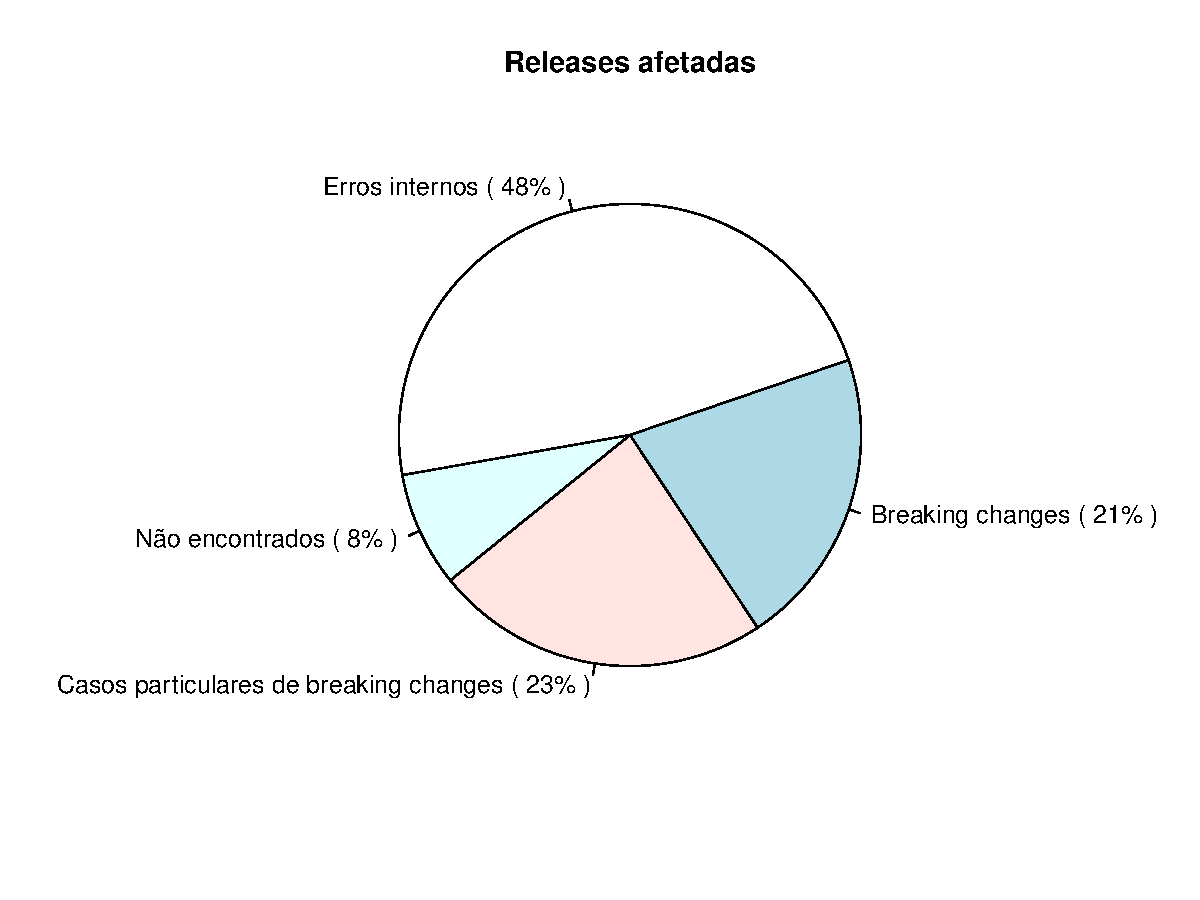
\includegraphics[scale=0.8]{figuras/pre_res_rq1.pdf}
    \caption{Resultado dos casos de erros em função das \textit{releases}.}
    \label{fig:pre_res_rq1}
\end{figure}{}

\subsubsection{Relação das \textit{releases} do cliente com os provedores e as \textit{breaking changes}}

Após analisar todos os casos de testes que resultaram em erro, foram constatados um total de 40 (10.4\%) clientes impactados por \textit{breaking changes}. Esses clientes sofreram com \textit{breaking changes} em pelo menos uma de suas \textit{releases}. Desde clientes com os testes executados em apenas uma \textit{release}, até os clientes com mais de 100 \textit{releases} foram impactados e, de maneira análoga, clientes com 1 provedor até clientes com mais de 100 provedores também foram impactados por \textit{breaking changes}. Observando apenas a amostra, é possível verificar que há uma correlação entre o número de \textit{releases} e o número de provedores, conforme a Figura \ref{fig:correlation_release_providers} apresenta. Nessa Figura, cada ponto representa um cliente com sua determinada quantidade de provedores e de \textit{releases}, respectivamente nos eixos \textit{x} e \textit{y}, também há uma regressão não-linear que caracteriza a correlação entre a quantidade de provedores e a quantidade de \textit{releases} que tiveram os testes executados, e por fim, há uma linha vertical e uma horizontal significando a mediana das \textit{releases} e dos provedores da amostra, respectivamente, sendo que essas medianas valem 3 e 9, assim, dividindo o plano cartesiano em 4 quadrantes. \daniel{havia alguns outliers que influenciavam um pouco no valor, mas usando um boxplot e um violin plot eu percebi que seria melhor usar a mediana à media. Mas a media daria 6 e 12}

Através da regressão não-linear percebe-se uma correlação entre o número de \textit{releases} e de provedores. Essa correlação caracteriza um crescimento no número de provedores a medida que o número de \textit{releases} aumenta, assim, quanto maior o número de \textit{releases}, maior o número de provedores que os clientes terão. Essa correlação também pode ser visualizada no quadrante em que estão os clientes que contêm seus provedores abaixo da mediana e suas \textit{releases} acima da mediana (inferior direito). Esse é o quadrante com a menor concentração de clientes, contendo apenas 7\%, e, visivelmente, percebe-se que, conforme as \textit{releases} aumentam, o número de provedores aumenta, tanto que o maior cliente contém 40 \textit{releases}, e os clientes que contém mais de 40 \textit{releases} possuem uma quantidade de provedores acima da mediana.

\begin{figure}
    \centering
    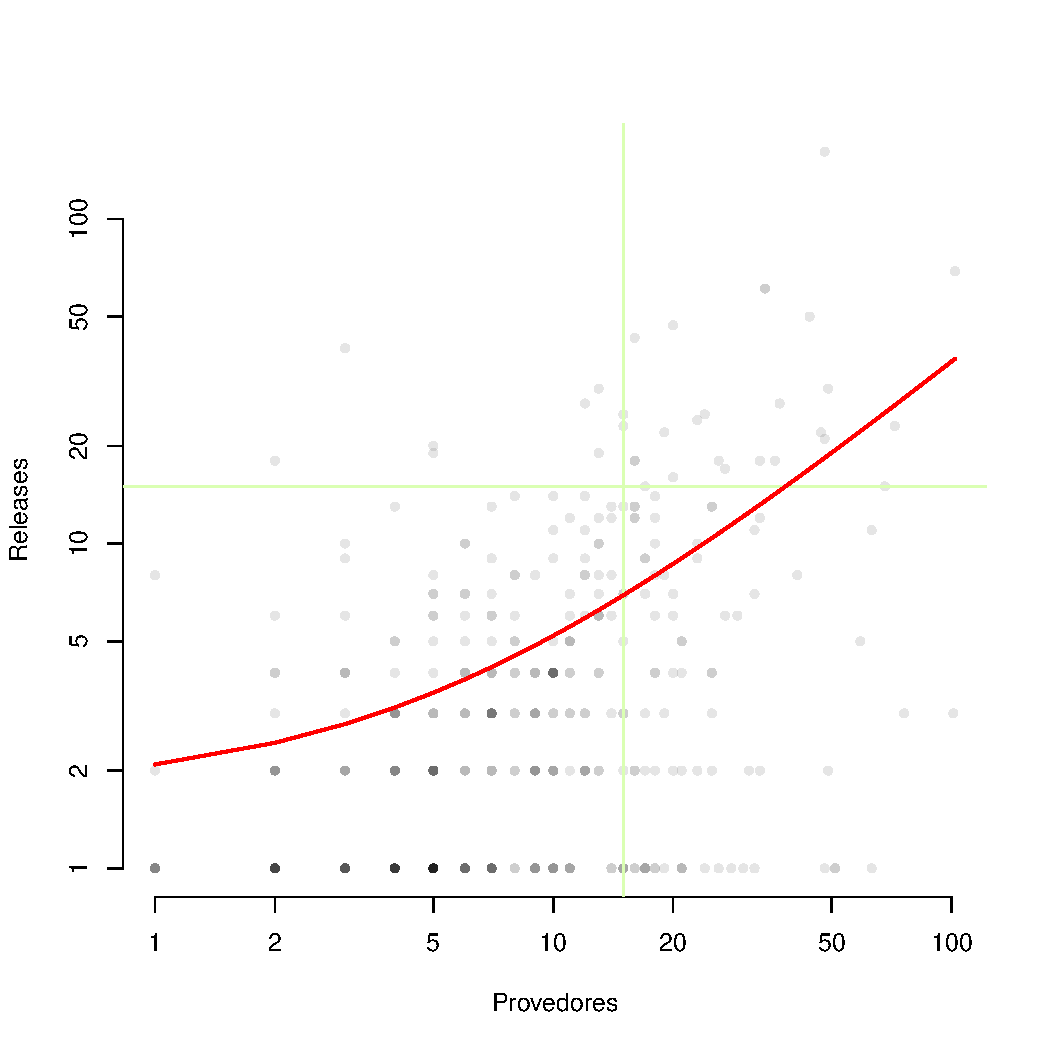
\includegraphics[scale=0.6]{figuras/correlation_release_providers.pdf}
    \caption{Correlação entre a quantidade de \textit{releases} e de provedores da amostra}
    \label{fig:correlation_release_providers}
\end{figure}{}

A análise dos clientes com \textit{breaking changes} se encontra na Figura \ref{fig:result_rq1_releases_affecteds}, que correlaciona a quantidade de provedores com a quantidade de \textit{releases} que foram executados os testes, respectivamente no eixo \textit{y} e \textit{x}. Nessa Figura, assim como na Figura anterior, estão dispersos os clientes da amostra e, em destaque, os que sofreram com \textit{breaking changes}. O tamanho dos círculos  representam a proporção de \textit{releases} dos clientes que foram impactadas, ou seja, a quantidade de \textit{releases} com os testes executados pela quantidade de \textit{releases} impactadas por \textit{breaking changes}. Assim, quanto maior os círculos vermelhos, maior o impacto das \textit{breaking changes}. Por fim, há uma regressão não-linear da relação dos provedores com as \textit{releases} dos clientes afetados com \textit{breaking changes} e uma linha vertical e uma horizontal significando a mediana das \textit{releases} e dos provedores que foram impactados por \textit{breaking changes}, respectivamente, e essas medianas valem 8 e 14, assim, dividindo o plano cartesiano em 4 quadrantes. A Figura \ref{fig:percentage_clients_bc} contém a porcentagem de clientes de cada quadrante da Figura \ref{fig:result_rq1_releases_affecteds}. Por exemplo, o quadrante superior esquerdo da Figura \ref{fig:result_rq1_releases_affecteds} contém 17.2\% dos clientes da amostra, como pode ser visto no seu respectivo eixo (\textit{Sup. esquerdo}) na Figura \ref{fig:percentage_clients_bc}, e desses 17.2\%, 10.6\% foram afetados com \textit{breaking changes}, ou seja, esses 10.6\% são a porcentagem de clientes impactados por \textit{breaking changes} nesse determinado quadrante.

\begin {figure} [h!]
   \centering
   \mbox {
        \subfigure[]{\label{fig:result_rq1_releases_affecteds} 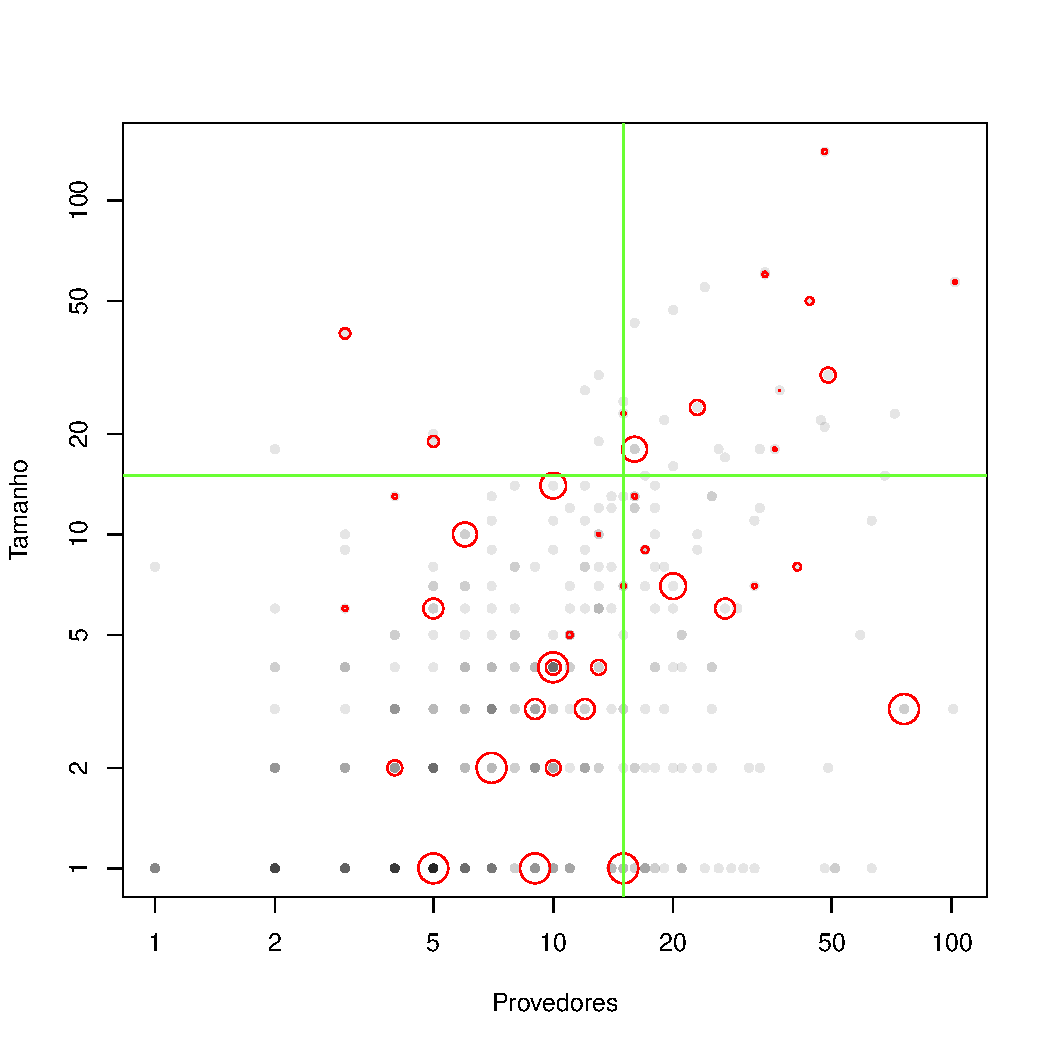
\includegraphics[scale=0.45]{figuras/result_rq1_releases_affecteds.pdf}}\quad
        \subfigure[]{\label{fig:percentage_clients_bc} 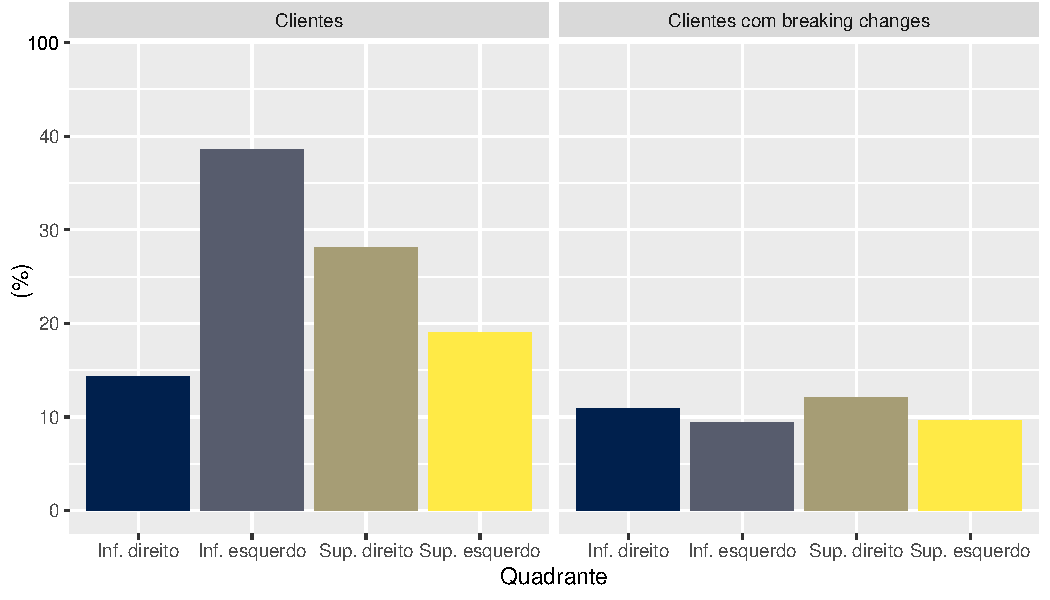
\includegraphics[scale=0.3]{figuras/percentage_clients_bc.pdf}}
    }
    \caption{(a) Quantidade de pacotes/\textit{releases} afetados pelo número de casos de \textit{break change}; (b) percentual de clientes em cada quadrante da Figura \ref{fig:result_rq1_releases_affecteds}}
    \label{fig:result_rq1_once_twice_three}
\end{figure}

Através da regressão não-linear da Figura \ref{fig:result_rq1_releases_affecteds}, verifica-se que a manifestação das \textit{breaking changes} está relacionada com o número de \textit{releases} executadas e com o número de provedores, uma vez que a regressão é crescente conforme a quantidade de provedores e de \textit{releases} aumentam. Mas, no quadrante em que há a maior concentração de clientes (inferior esquerdo), com 64.6\% dos clientes da amostra, há a mais baixa porcentagem de casos de \textit{breaking changes}, com um total de 5.6\% de ocorrências, mesmo sendo o quadrante com mais clientes. Neste caso, conclui-se que a manifestação de \textit{breaking changes} para clientes com um quantidade abaixo da mediana de provedores e de \textit{releases} não é comum, ou seja, os clientes com poucos provedores e poucas \textit{releases} foram os menos impactados. Ainda analisando a Figura \ref{fig:percentage_clients_bc}, é possível verificar que a manifestação de \textit{breaking changes} está fortemente relacionada com a quantidade de \textit{releases} do cliente. Essa relação está no fato de que os quadrantes com os maiores percentuais de ocorrência de \textit{breaking changes} são os quadrantes \textit{superior direito} e \textit{inferior direito}, com 30.2\% e 22.2\% de seus clientes impactados, respectivamente, e a Figura \ref{fig:result_rq1_releases_affecteds} mostra que esses dois quadrantes são os que possuem os clientes com a quantidade de \textit{releases} acima da mediana. E, como a quantidade de \textit{releases} que tiveram seus testes executados está diretamente relacionada com as atualizações dos provedores -- as \textit{releases} só foram executadas quando havia algum provedor que tinha atualizado --, conclui-se que a manifestação das \textit{breaking changes} é motivada pela frequência com que os provedores publicam suas \textit{releases}. Clientes que possuem grande quantidade de provedores, mas que possuem poucas \textit{releases} com seus testes executados, não são tão impactados por \textit{breaking changes} quanto os clientes que tiveram uma grande quantidade de \textit{releases} com testes executados.


% a baixa quantidade de amostras para os dois e três casos de break changes deixou esta conclusão um pouco estranha e meio "não-genérica"
\subsubsection{Variedade de \textit{breaking changes} nos pacotes}
As \textit{break changes} são imprevisíveis. Elas ocorrem independentemente uma das outras, ou seja, um pacote pode ser impactado com apenas um caso de \textit{break change}, mas também pode ser impactado com mais de um caso. E foi isso o que aconteceu: dos 40 pacotes afetados, 35 (87.5\%) foram impactados por apenas um caso de \textit{break change} e 5 (12.5\%) foram impactados por mais de um caso, sendo que 4 (10\%) foram impactados por dois casos e 1 (2.5\%) pacote sofreu a manifestação de 3 casos de \textit{breaking change}. A Figura \ref{fig:result_rq1_once_twice_three_1} contém estes dados.

\begin {figure} [h!]
   \centering
   \mbox {
        \subfigure[]{\label{fig:result_rq1_once_twice_three_1} 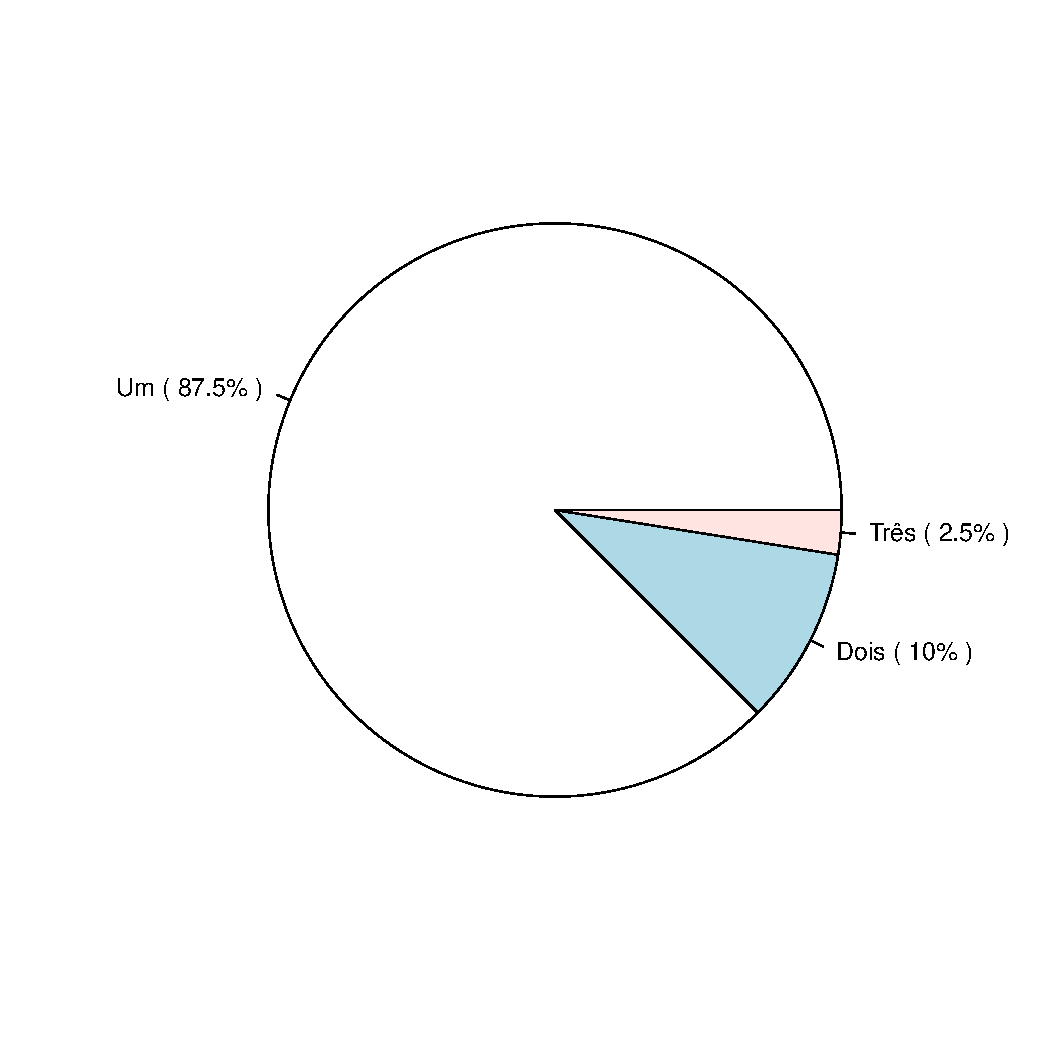
\includegraphics[scale=0.4]{figuras/result_rq1_once_twice_three_1.pdf}}\quad
        \subfigure[]{\label{fig:result_rq1_once_twice_three_2} 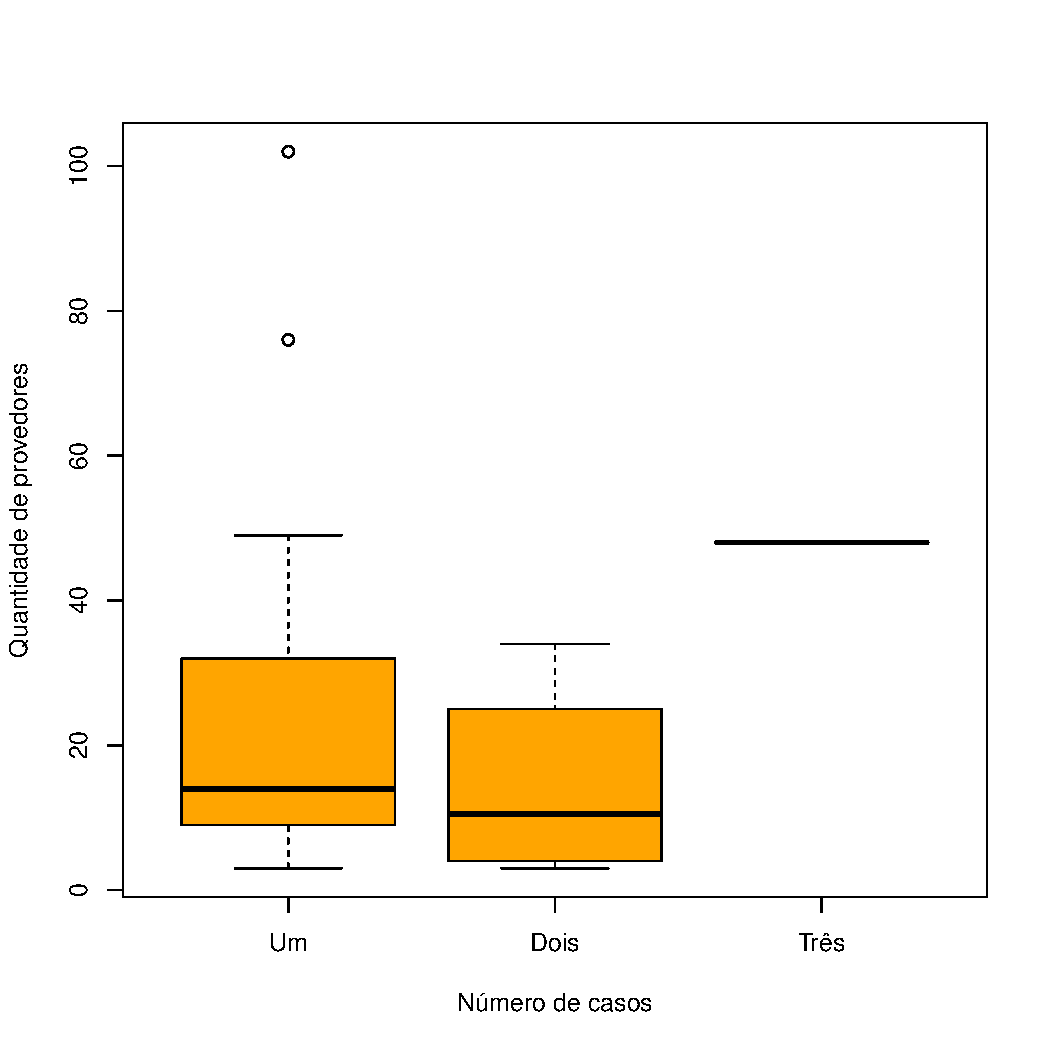
\includegraphics[scale=0.45]{figuras/result_rq1_once_twice_three_2.pdf}}
    }
    \caption{Quantidade de pacotes/\textit{releases} afetados pelo número de casos de \textit{break change}}
    \label{fig:result_rq1_once_twice_three}
\end{figure}

A Figura \ref{fig:result_rq1_once_twice_three_2} apresenta três \textit{boxplots} da quantidade de provedores que cada pacote possui em relação à quantidade de casos de \textit{breaking changes} sofridos. O único pacote que foi impactado por três casos de \textit{breaking change} é o que contém o maior número de \textit{releases} e, mesmo apresentando a menor proporção de casos afetados de acordo com a Figura \ref{fig:result_rq1_once_twice_three_1}, ele possui a maior mediana de provedores que os demais. Nesse caso, três provedores diferentes causaram os três casos de \textit{breaking changes} e por isso a quantidade de provedores favoreceu a ocorrência dos três casos, uma vez que a quantidade de \textit{releases} não fator determinante, visto a proporção na Figura \ref{fig:result_rq1_once_twice_three_1}. \filipe{Precisa fazer um teste de hipótese e calcular effect size para confirmar o que você está dizendo. Outra coisa é mostrar esse gráfico como um beanplot cortado ao meio. Não acho que o terceiro boxplot seja necessário, só tem um data point nele, não é isso? Dá pra descrever no texto.}\daniel{Ok, vou fazer um teste de hipóste e um effect size, mas o não entendi se o senhor quer um beanplot ali?} Um fato é que a ocorrência de mais de um caso de \textit{breaking changes} não é tão comum, pois os pacotes que foram impactados por dois casos possuem uma mediana de provedores menor do que os pacotes que foram impactados por apenas um caso.

%\subsubsection{Impacto dos provedores indiretos}
%O \textit{npm} contém a maior rede de dependências entre os pacotes dentre os principais repositórios, conforme explicado na Seção \ref{ref-teo:npm}. Nesse emaranhado de projetos dependendo mutuamente uns dos outros, não é difícil pressupor que não somente os provedores diretos podem introduzir as \textit{break changes}. Assim como o cliente usa o provedor direto, o provedor indireto é usado da mesma maneira pelo provedor direto, fazendo do provedor indireto um indivíduo muito influente para a execução do cliente.

\section{RQ2. Como os pacotes provedores introduzem \textit{breaking changes} em uma \textit{release}?}


\subsubsection{Categorias de \textit{Breaking changes}}
Ao todo, foram 43 casos de \textit{breaking changes} distribuídas em 39 clientes diferentes. Todos esses casos foram agrupados em 8 diferentes categorias das quais se encaixavam. A Tabela \ref{tab:bc_category} apresenta cada uma dessas categorias, bem como a quantidade de pacotes e a quantidade de \textit{releases} que cada categoria atingiu.

\begin{table}[]
\begin{tabular}{|l|c|c|c|c|}
\hline
\centering
\textbf{Categoria}           & \textbf{Pacotes afetados} & \textbf{\%}   & \textbf{\textit{Release} afetadas} & \textbf{\%}    \\ \hline
Alteração de regras          & 12              & 27,9 & 64                          & 33,68 \\
Provedores incompatíveis     & 8               & 18,6 & 30                          & 15,78 \\
Alteração de tipo de objeto  & 8               & 18,6 & 24                          & 12,63 \\
Objeto indefinido            & 4               & 9,3  & 25                          & 13,15 \\
Código errado                & 4               & 9,3  & 13                          & 6,84  \\
Código não-atualizado        & 3               & 6,97 & 25                          & 13,15  \\
Renomeação de função         & 3               & 6,97 & 5                           & 2,63  \\
Arquivo não encontrado       & 1               & 2,32 & 4                           & 2,1  \\ \hline
\textbf{Total}               & 43              &      & 190                         &       \\ \hline
\end{tabular}
\caption{Categorias dos casos de \textit{break change}}
\label{tab:bc_category}
\end{table}

A seguir, encontra-se uma descrição sobre cada categoria e um exemplo de como os pacotes dessa determinada categoria foram afetadas.

\begin{itemize}
    \item \textbf{Alteração de regras}: este caso foi o principal que impactou os pacotes. Essa categoria contém os casos de \textit{break change} no qual os provedores possuíam um determinado comportamento, mas alteraram algumas de suas regras/funcionalidades e impactaram os seus clientes. Não foi uma simples alteração no código, tal como uma alteração de tipo de variáveis, ou um código escrito de maneira errada, mas sim uma regra no qual o cliente tinha como sólida, foi alterada. Por exemplo, o pacote \textit{request@2.17.0} -- essa \textit{release} não existe mais no \textit{npm}, mas a alteração se manteve -- introduziu uma alteração em seu código\footnote{https://github.com/request/request/commit/d05b6ba72702c2411b4627d4d89190a5f2aba562\#diff-168726dbe96b3ce427e7fedce31bb0bcR857}, como pode ser visto na Figura \ref{fig:bc_category_change_rule_1}.

    \begin{figure}
        \centering
        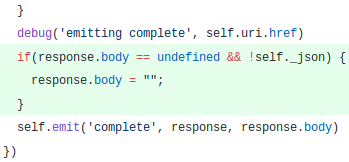
\includegraphics[scale=0.6]{figuras/bc_category_change_rule_1.png}
        \caption{Alteração de regra de funcionamento do \textit{request}}
        \label{fig:bc_category_change_rule_1}
    \end{figure}{}

    Nesse caso, o \textit{request} adiciona uma \textit{string} vazia ao invés de manter \textit{undefined} o corpo de uma requisição. Esse caso do \textit{request} ocorreu exatamente como foi explicado por \citeonline{Foo:2018:ESC:3236024.3275535} dizendo que os pacotes evoluem independentemente dos clientes. Essa alteração na regra do \textit{request} reflete em uma evolução do pacote, mas o cliente não esperava essa alteração e confiava que o corpo da resposta fosse retornado como \textit{undefined} em caso de erro, por isso o cliente quebrou.

    \item \textbf{Provedores incompatíveis}: nessa categoria, há um provedor direto A e um provedor indireto B envolvido, o qual alterou o seu código, o que não gerou um erro, mas provocou no provedor A um comportamento inesperado, ou seja, o provedor B passou a ser incompatível com o provedor A. Nessa categoria, nenhum dos provedores contém um erro, mas sim uma incompatibilidade. Um exemplo disso ocorreu com os pacotes \textit{babel-eslint}\footnote{https://www.npmjs.com/package/babel-eslint} e \textit{escope}\footnote{https://www.npmjs.com/package/escope}, sendo o pacote \textit{escope} é um provedor indireto do \textit{babel-eslint}.

    \begin{figure}
        \centering
        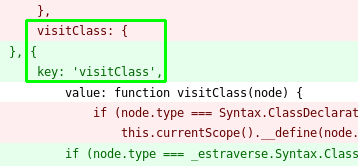
\includegraphics[scale=0.5]{figuras/bc_category_incompatibles_providers.png}
        \caption{Alteração de código do \textit{escope}}
        \label{fig:bc_category_incompatibles_providers}
    \end{figure}{}

    A \textit{releases escope@3.4} realizou uma alteração no seu código, de acordo com a Figura \ref{fig:bc_category_incompatibles_providers}, mas que não reflete em um erro. Essa alteração impactou diretamente o pacote \textit{babel-eslint}, mesmo o pacote \textit{escope} não sendo um provedor direto do \textit{babel-eslint} e não ter introduzido um erro\footnote{https://github.com/estools/escope/issues/99\#issuecomment-178151491}. Com isso, há uma incompatibilidade entre os provedores e essa incompatibilidade precisou ser corrigida pelo \textit{babel-eslint} e não pelo \textit{escope}. Essa foi a \textit{breaking change} que mais surgiu na análise manual pois, dos 43 casos, 5 (11.6\%) refletiam essa incompatibilidade, uma vez que o \textit{babel-eslint} é provedor direto de 5.8\% de toda o conjunto de dados.

    \item \textbf{Alteração de tipo de objeto}: essa é uma categoria de \textit{break changes} facilmente detectável em linguagens fortemente tipadas, mas no \textit{Javascript} representam um tipo de \textit{break change} que, por muitas vezes, pode nem afetar o código do cliente. Mas, neste trabalho, foram detectados 8 (18.6\%) de casos nos quais os provedores alteraram o tipo de alguma variável.

    \begin{figure}
        \centering
        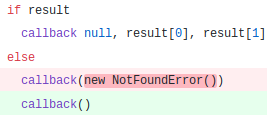
\includegraphics[scale=0.5]{figuras/bc_category_change_type.png}
        \caption{Alteração de um tipo \textit{array} para \textit{object}}
        \label{fig:bc_category_change_type}
    \end{figure}{}

    Na Figura \ref{fig:bc_category_change_type} o provedor \textit{socket.io}\footnote{https://www.npmjs.com/package/socket.io} alterou alguns \textit{arrays} para \textit{object}\footnote{https://github.com/socketio/socket.io/commit/b73d9bea4efb48277eee685763026ff2df5a79ab}. Anteriormente, os clientes iteravam nesses \textit{arrays}, mas após essa alteração, os clientes foram afetados.

    \item \textbf{Objeto indefinido}: por vezes, os códigos podem estar todos corretos, mas então o provedor tenta acessar uma variável que não existe. Esta categoria de \textit{break change} representa os casos no qual os provedores tentaram obter acesso à alguma variável/objeto, mas que não existiam. Esses erros são os que facilmente podem ser consertados/evitados apenas adicionando o código da Listagem \ref{cod:undefined_object}:

    \begin{lstlisting}[style=bash, label=cod:undefined_object]
    this.var = this.var || {};
    \end{lstlisting}

    Esse tipo de erro surgiu no pacote \textit{ember-cli-htmlbars-inline-precompile}\footnote{https://www.npmjs.com/package/ember-cli-htmlbars-inline-precompile}, no qual o desenvolvedor tenta acessar uma variável que não estava disponível. Mas, assim como o desenvolvedor já havia feito com as demais variáveis da Figura \ref{fig:bc_category_undefined_object}, uma simples alteração no código foi o suficiente.

    \begin{figure}
        \centering
        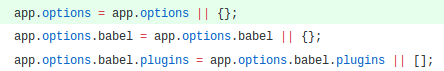
\includegraphics[scale=0.7]{figuras/bc_category_undefined_object.png}
        \caption{Correção do erro de objeto indefinido}
        \label{fig:bc_category_undefined_object}
    \end{figure}{}

    \item \textbf{Código errado}: este caso de \textit{break change} ocorreu quando o provedor escreveu um código semanticamente incorreto, gerando um erro na sua execução e afetando o cliente. Em linguagens compilada, esse tipo de erro seria facilmente identificado pelo compilador em tempo de compilação. Foi exatamente isso que a dependência fez. Ao alterar o seu código, o desenvolvedor escreveu duas vezes a mesma variável, como pode ser visto na Figura \ref{fig:bc_category_wrong_code}. Assim como os erros do tipo \textit{undefined object}, os erros dessa categoria  são facilmente corrigidos.

    \begin{figure}
        \centering
        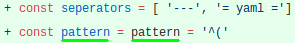
\includegraphics[scale=0.8]{figuras/bc_category_wrong_code.png}
        \caption{Código semanticamente incorreto}
        \label{fig:bc_category_wrong_code}
    \end{figure}{}

    \item \textbf{Renomeação de função}: as \textit{break changes} relacionadas à esta categoria foram facilmente detectáveis. Quando a mensagem de erro do \textit{node.js} era exibida como \textit{TypeError: var is not a function}, com pouca investigação já era possível saber que uma determinada função não estava mais disponível, ou seja, havia sido removida ou alterado o seu nome.

    \begin{figure}
        \centering
        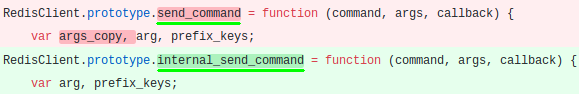
\includegraphics[scale=0.6]{figuras/bc_category_renamed_function.png}
        \caption{Alteração do nome de função}
        \label{fig:bc_category_renamed_function}
    \end{figure}{}

    \item \textbf{Arquivo não encontrado}: os casos de \textit{break change} relacionados à esta categoria são aqueles no qual o desenvolvedor realiza um acesso a um arquivo, mas esse não existe. O arquivo requerido pode não existir ou não estar disponível, uma vez que, referenciado no arquivo \textit{.npmignore} -- arquivo utilizado pelo \textit{npm} para ignorar arquivos durante o processo de publicação --, o arquivo existe mas não está disponível, mas também o arquivo pode não existir. Entretanto, o único caso de arquivo não encontrado ocorreu pois o arquivo \textit{index.js} estava indisponível. O provedor \textit{esprima-extract-comments}\footnote{https://www.npmjs.com/package/esprima-extract-comments} utilizava como provedor um \textit{fork} do pacote \textit{esprima}\footnote{https://github.com/ariya/esprima/} e o referencia em seu  \textit{package.json} para ser descarregado diretamente do \textit{Github}\footnote{https://github.com/jonschlinkert/esprima-extract-comments/blob/6b65a0f52f85bc6fa830d44e352ec3da9e9ef620/package.json\#L47}. Entretanto, o \textit{index.js} desse \textit{fork}, foi referenciado no \textit{.gitignore} e não estava disponível quando o \textit{npm} descarregou o pacote diretamente do \textit{Github}, mas o arquivo estava disponível se o pacote \textit{exprima} fosse descarregado diretamente do \textit{npm}.

\end{itemize}{}

\section{RQ3. Como os pacotes clientes se recuperam das \textit{breaking changes}?}








